\section{Experiment 3. 07.02.2020}\label{experiment-3.-07.02.2020}

Took place on 27.02.2020

This time the aim was to check how \textbf{2 major updates} of the Android app behave.

The \emph{first} one concerned the usage of HTTP requests instead of MQTT. The reason for it is that all previously detected issues related to MQTT in one way or another.

The \emph{second} update was about complete refactoring of the code. It included not only start following MVVM architectural pattern but also removing of redundant `Connect' button, then real-time interaction with the app coordinates updates the display when `Push continuously' enabled.

\subsection{Procedure}

Due to the bad weather (heavy snowfall), we decided to experiment indoor (Mensa building in TU Ilmenau has enough space inside). 1 CnC, 1 AP, and 3 UEs took part.

All UEs can connect successfully:

\begin{itemize}
\tightlist
\item
  `Push once' button pressed
\item
  deviceId assigned
\item
  UE coordinates displayed
\end{itemize}

\subsection{Tips}

As for `Push continuously', it should be known in advance the
coordinates updated on the display \textbf{only in the case of moving to
some minimal delta} (10 centimeters). This is insured based on GPS
values passed by the Android device.

To make sure the connection is still alive, and the values are transferred, it makes sense to check logging messages in logs/log.txt in UE.

\subsection{Outcome}

To sum up, the system finally started working as expected, and the meaningful set of data is collected, as shown in the following figures.

\begin{figure}[H]
	\centering
	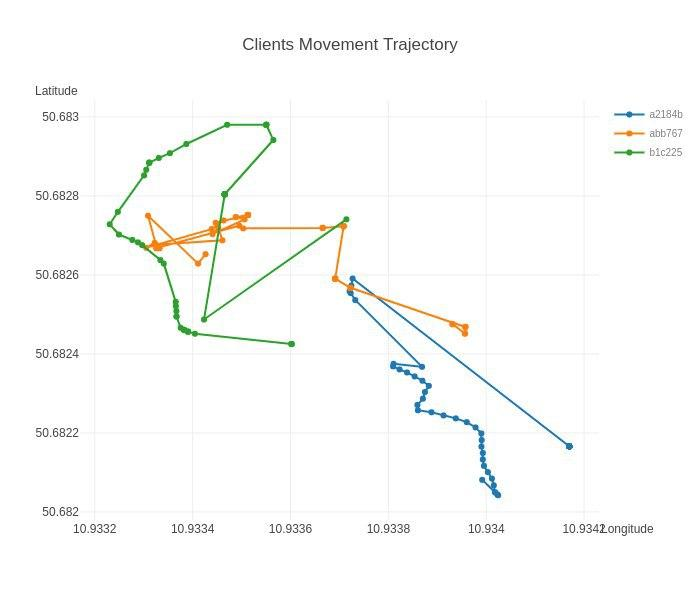
\includegraphics[width=\linewidth,keepaspectratio]{images/experiment_3_1.jpg}
\caption{Movement trajectory of connected phones}
\end{figure}

\begin{figure}[H]
	\centering
	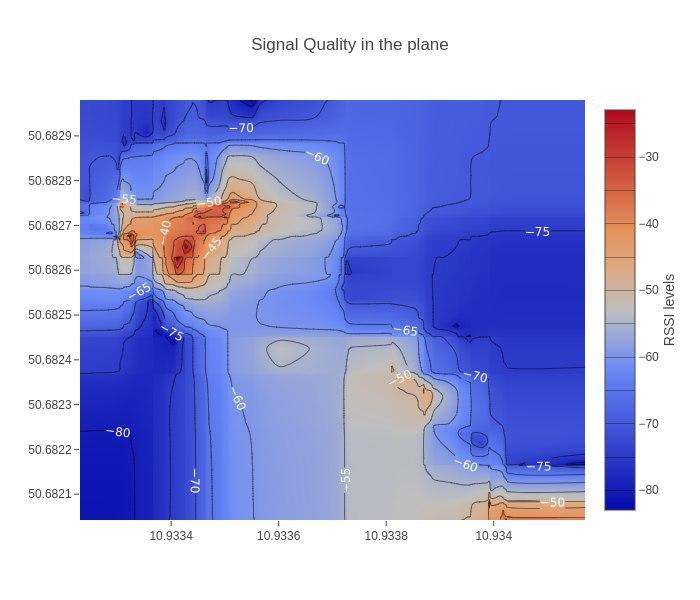
\includegraphics[width=\linewidth,keepaspectratio]{images/experiment_3_2.jpg}
\caption{Signal quality map}
\end{figure}

\begin{figure}[H]
	\centering
	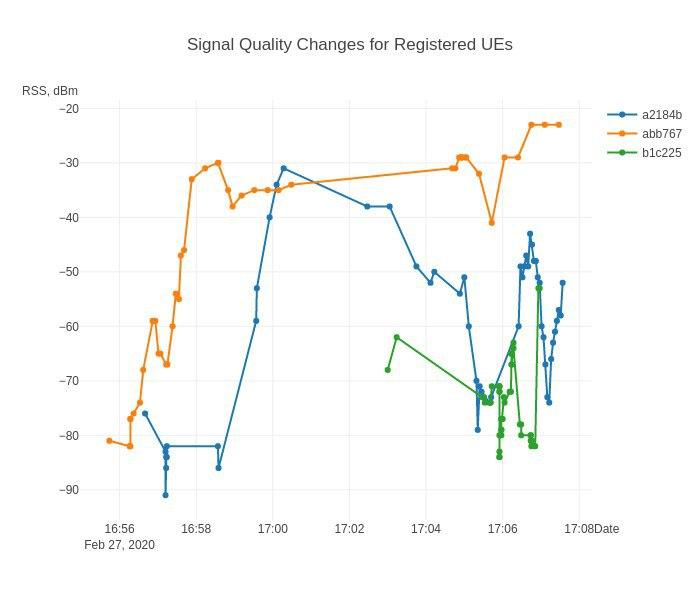
\includegraphics[width=\linewidth,keepaspectratio]{images/experiment_3_3.jpg}
\caption{Signal quality changes}
\end{figure}
